\documentclass[11pt, aspectratio=169, compress]{beamer}
\usetheme[progressbar=frame title, numbering=fraction]{metropolis}      % Use metropolis theme 
\setbeamertemplate{section in toc}[sections numbered]
\setbeamertemplate{subsection in toc}[subsections numbered]
\useoutertheme[subsection=false]{miniframes}
\setbeamercolor{section in head/foot}{fg=white, bg=mDarkTeal}
\setbeamercolor{background canvas}{bg=white}
\setbeamerfont{section in head/foot}{series=\bfseries}

\usefonttheme[onlymath]{serif}
\usepackage{amsmath}
\usepackage{remreset}
\usepackage{ragged2e}
\usepackage{booktabs}
\usepackage{makecell}
\usepackage{float}
\usepackage{subfig}
\usepackage{tikz}
\usetikzlibrary{positioning,calc}
\usepackage[flushleft]{threeparttable}	% 3 part table 
\usepackage[justification=centering]{caption}
\captionsetup{skip=0pt}
\graphicspath{{./fig/}}

\makeatletter
\let\beamer@writeslidentry@miniframeson=\beamer@writeslidentry
\def\beamer@writeslidentry@miniframesoff{%
	\expandafter\beamer@ifempty\expandafter{\beamer@framestartpage}{}% does not happen normally
	{%else
		% removed \addtocontents commands
		\clearpage\beamer@notesactions%
	}
}
\newcommand*{\miniframeson}{\let\beamer@writeslidentry=\beamer@writeslidentry@miniframeson}
\newcommand*{\miniframesoff}{\let\beamer@writeslidentry=\beamer@writeslidentry@miniframesoff}
\beamer@compresstrue
\makeatother

%==============================================================
% Title Page
%==============================================================
%Information to be included in the title page:
\title{Economía social: programas y políticas de apoyo social}
\author{Rony Rodriguez-Ramírez} 
\institute{Economía Social y Humana | Grupo B018 \\Universidad Centroamericana}
\titlegraphic{\hfill
\includegraphics[height=1.5cm]{uca}}
\date{\today}
%==============================================================
\begin{document}
	
\begin{frame}[plain]
	\maketitle  
\end{frame}

%\begin{frame}{Outline}
%\tableofcontents[hideallsubsections]
%\end{frame}
%------------------------------------------------
\section{Comentarios y anuncios}
%-----------------------------------------------
\subsection{Comentarios y anuncios}
%-----------------------------------------------
\begin{frame}[t]{Comentario y anuncios}
\begin{itemize}
	\item Talleres. 
	\item Ensayo. 
	\item Papers en inglés. 
	\begin{itemize}
		\item Importancia. 
	\end{itemize}
\end{itemize}
\end{frame}
%------------------------------------------------
\section{La idea de la intervención social}
%------------------------------------------------
\subsection{Intervención y programas sociales}
%------------------------------------------------
\begin{frame}[t]{Conceptos claves} 
	Un componente interesante de la economía social es la intervención (social) que se da a través de programas o políticas públicas. 
	
	En general, las intervenciones tienen como objetivo: 
	\begin{itemize}
		\item un grupo en particular; 
		\item mejorar las condiciones de vida de esos grupos (responden a las necesidades de estos); 
		\item buscar un cambio social. 
	\end{itemize}
\end{frame}
%------------------------------------------------
\begin{frame}[t]{Intervenciones} 
En Nicaragua: 
\begin{itemize}
	\item Se estima que han habido alreador de 47 programas de asistencia social impulsados por elg obierno (Banco Mundial, 2017).
	\item Ha habido poca o nula evaluación de estos programas, y  tampoco hay mucha información pública. 
\end{itemize}
\end{frame}
%------------------------------------------------
\section{Intervenciones en educación: Head Start}
%------------------------------------------------
\subsection{El programa Head-Start}
%------------------------------------------------
\begin{frame}[t]{El programa Head Start}
	Uno de los programas más importantes en términos de evaluación es \textbf{Head Start} en los Estados Unidos. 
\begin{itemize}
	\item Es un program público pre-escolar para niños/as en desventajas. 
	\item Comenzó en 1965, como parte de la "guerra contra la pobreza" principalmente en apoyo a las comundiades afroamericanas. 
\end{itemize}	
\end{frame}
%------------------------------------------------
\begin{frame}[t]{El programa Head Start}
	Este tipo de intervenciones se relaciona con: 
	\begin{itemize}
		\item La teória del capital humano. 
		\item ¿Por qué se debería de invertir en los primeros años de los/las niños/as? 
	\end{itemize}	
\end{frame}
%------------------------------------------------
\begin{frame}[t]{El programa Head Start}
	Garces, Currie y Thomas (2002) utilizaron modelos de efectos fijos familiares para estimar el impacto del programa Head Start en varios resultados: 
	\begin{itemize}
		\item Probabilidad de completar la escuela secundaria, probabilidad de asistir a la universidad, ganancias y probabilidad de ser detenido o acusado de un delito. 
		\item Utilizan datos del Panel Study of Income Dynamics (PSID) que contiene información sobre las familias y los individuos en las familias. 
	\end{itemize}
\end{frame}
%------------------------------------------------
\begin{frame}[t]{El programa Head Start}
	\begin{itemize}
		\item Al evaluar el efecto de Head Start, deberíamos preocuparnos que las familias que envían a sus hijos a Head Start sean de alguna manera diferentes de las familias que no envían a sus hijos a Head Start.
		\item Garces et al. (2002) abordan este problema estimando modelos de efectos fijos familiares. 
		\item El papel de los efectos fijos familiares aquí es controlar las diferencias entre familias que no varían entre hermanos/as.
	\end{itemize}
\end{frame}
%------------------------------------------------
\begin{frame}[t]{El programa Head Start}
	\begin{itemize}
	\item El papel de los efectos fijos familiares aquí es controlar las diferencias entre familias que no varían entre los hermanos.
	\item Algunos componentes importances de los datos: 
	\begin{itemize}
	\item Algunas familias envían a todos sus hijos al programa (\textbf{tipo de familia 1}).
	\item Algunas familias no envían a ninguno de sus hijos (\textbf{tipo de familia 2}).
	\item Algunas familias envían algunos de sus hijos y otros no (\textbf{familia tipo 3}).
	\end{itemize}
	\item Los efectos fijos familiares nos permiten explotar la variación dentro de las familias, las estimaciones de los efectos fijos familiares se basan en el tercer tipo de familia. 
	\end{itemize}
\end{frame}
%------------------------------------------------
\begin{frame}[t]{El programa Head Start}
	\vspace*{-2.5ex}
	\begin{center}
	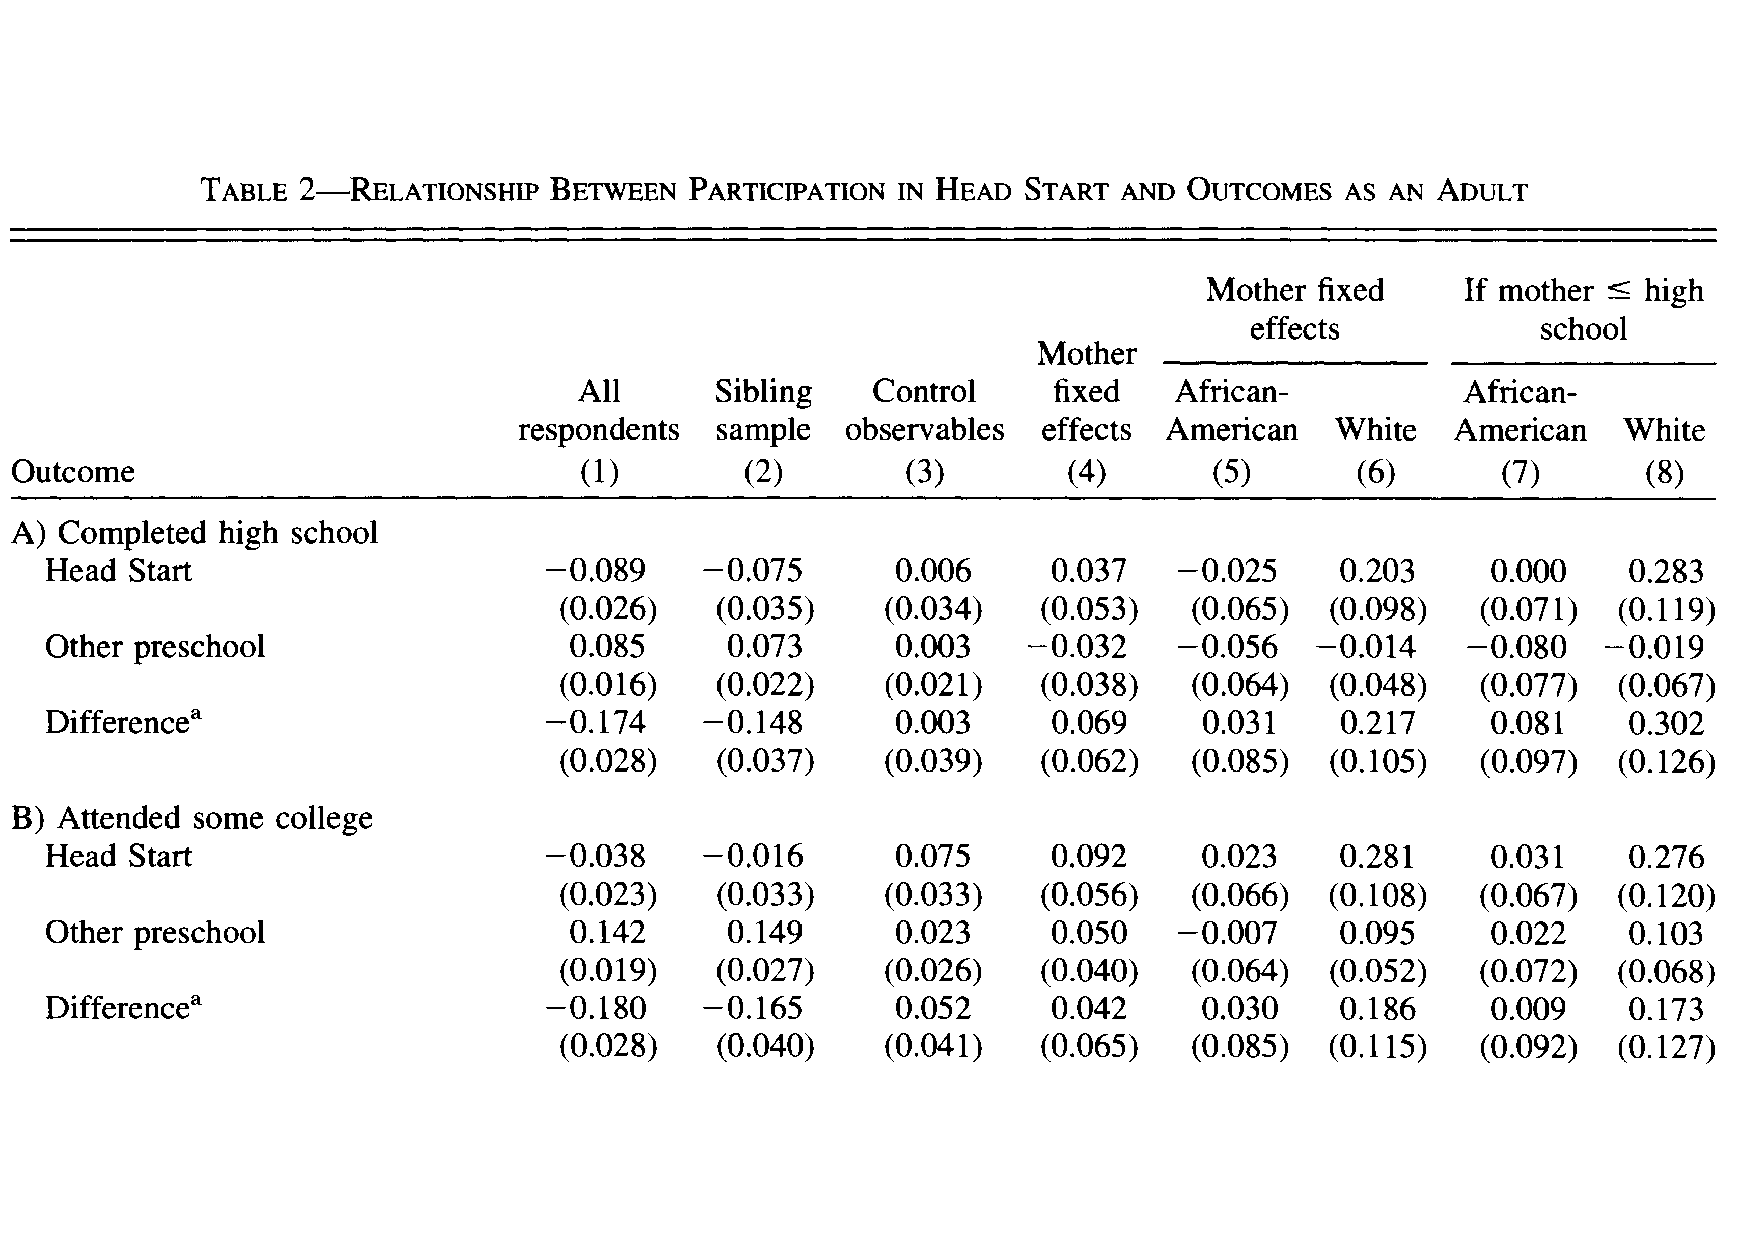
\includegraphics[width=0.8\textwidth]{tab1}
	\end{center} 
\end{frame}
%------------------------------------------------
\begin{frame}[t]{El programa Head Start}
	\vspace*{-2.5ex}
	\begin{center}
		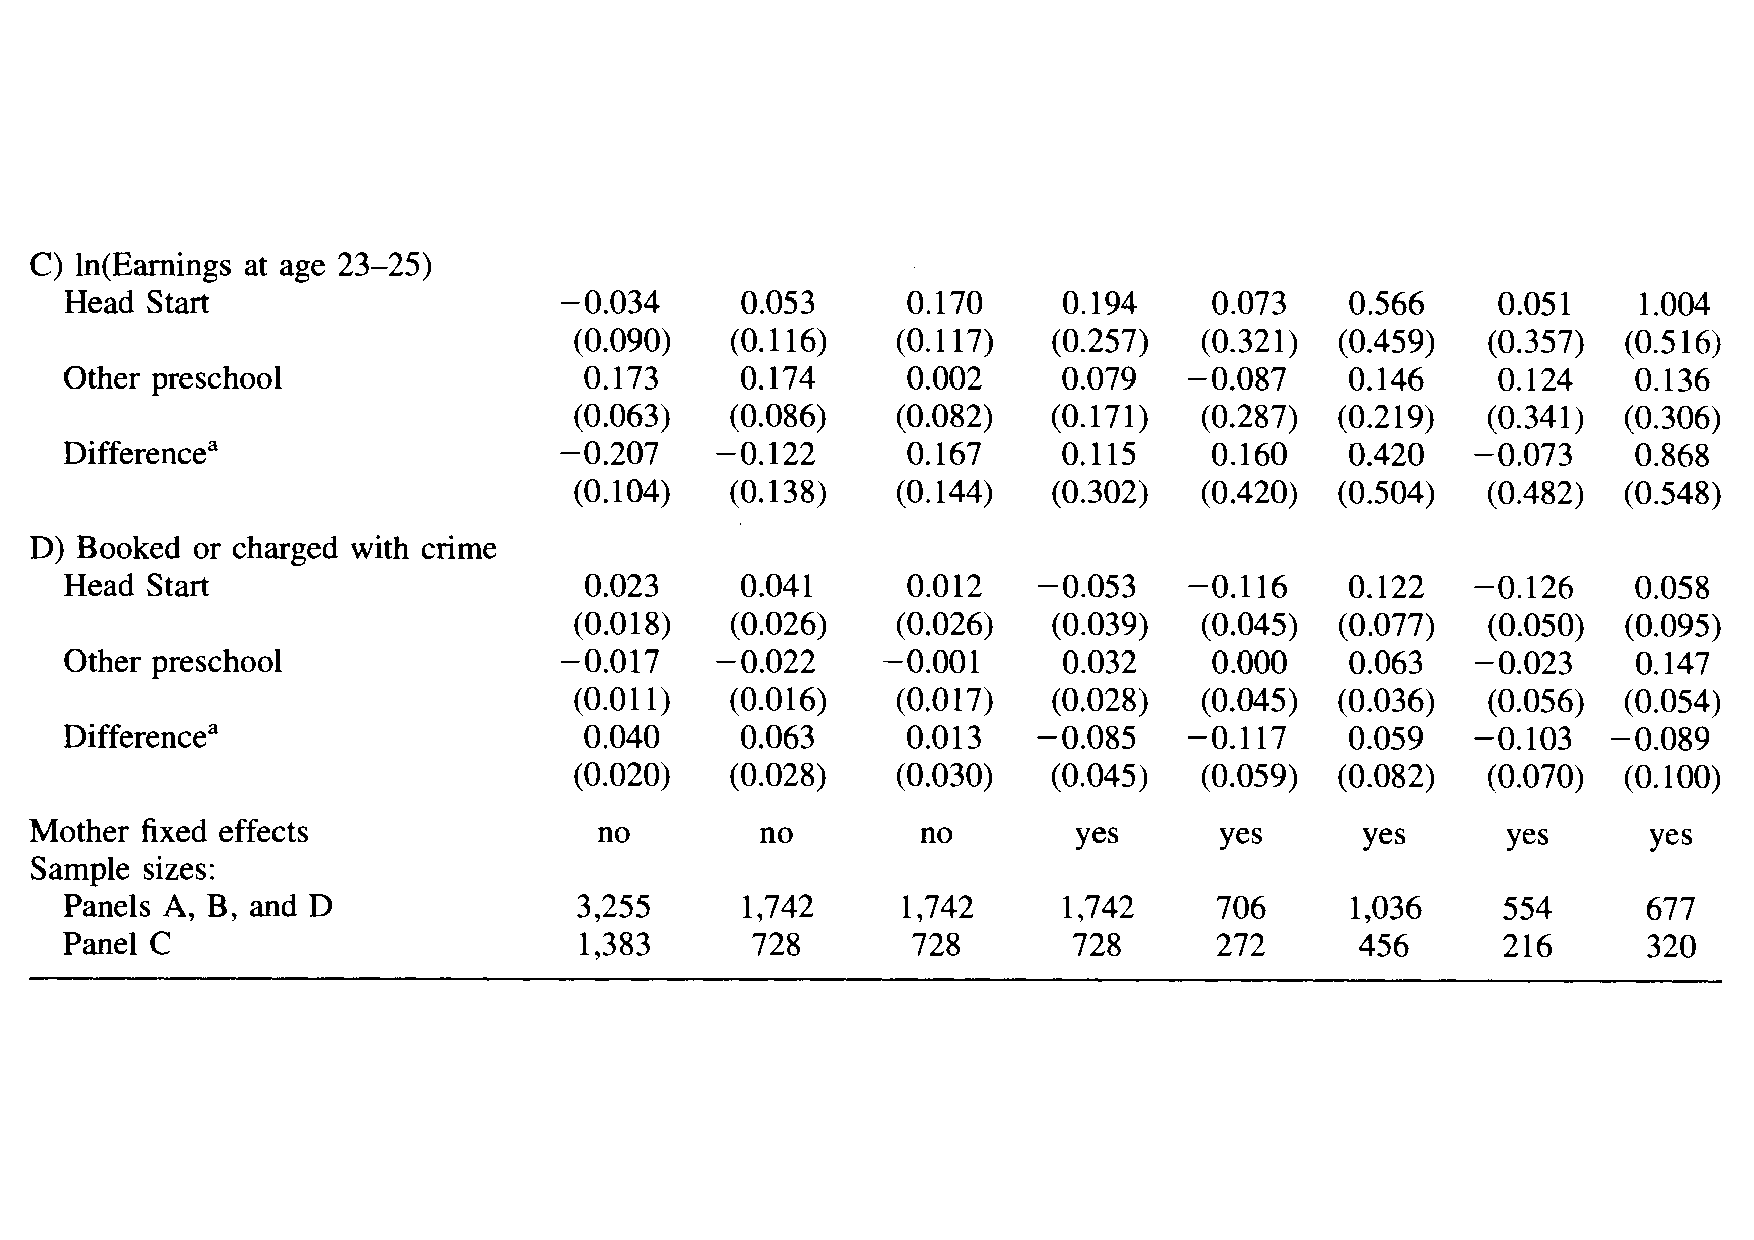
\includegraphics[width=0.8\textwidth]{tab2}
	\end{center} 
\end{frame}
%------------------------------------------------
\begin{frame}[t]{Conclusiones generales del program}
	\begin{itemize}
		\item La participación en Head Start tiene efectos positivos en la probabilidad de asistir a la universidad.
		\item Aumento en la probabilidad de graduarse de la escuela secundaria, y posiblemente en los ingresos como adultos jóvenes. 
		\item Afroamericanos que participaron en Head Start tienen significativamente menos probabilidades de haber sido registrados o acusados de un delito.
	\end{itemize}
\end{frame}
%------------------------------------------------
\section{Diseño de políticas públicas}
\subsection{Diseño de políticas públicas}
%------------------------------------------------
\begin{frame}[t]{Diseño de políticas públicas}
	Las políticas públicas también se pueden ver como intervenciones sociales, sobre todo porque hay: 
	\begin{itemize}
		\item un grupo de interes, el cual es el sujeto de la política;  
		\item un objetivo de política; 
		\item se busca un cambio social. 
	\end{itemize}
	Sin embargo, también resulta difícil ver el impacto de estas políticas; especialmente cuando no se diseñan con ese objetivo. 
\end{frame}
%------------------------------------------------
\begin{frame}[t]{Diseño de políticas públicas}
	Algunos ejemplos de políticas públicas que han servido como soporte social: 
	\begin{itemize}
		\item \textbf{Educación}: Creación e inversión en escuelas; programas de asistencia educativa. Leyes de educación obligatoria. 
		\item \textbf{Salud}: Provisión de servicios de salud a bajo costo, leyes de acceso a anticonceptivos. 
		\item \textbf{Mercado Laboral}: Asistencia técnica, transferencias a personas desempleadas. 
		\item \textbf{Política}: Cuota de representación para las mujeres. 
	\end{itemize}
	En esta semana nos dedicaremos a estudiar algunos de estos ejemplo, comenzado esta semana con salud. 
\end{frame}
%------------------------------------------------
\section{Políticas en salud}
\subsection{Políticas en salud}
%------------------------------------------------
\begin{frame}[t]{Intervenciones en salud: necesidad}
\begin{center}
	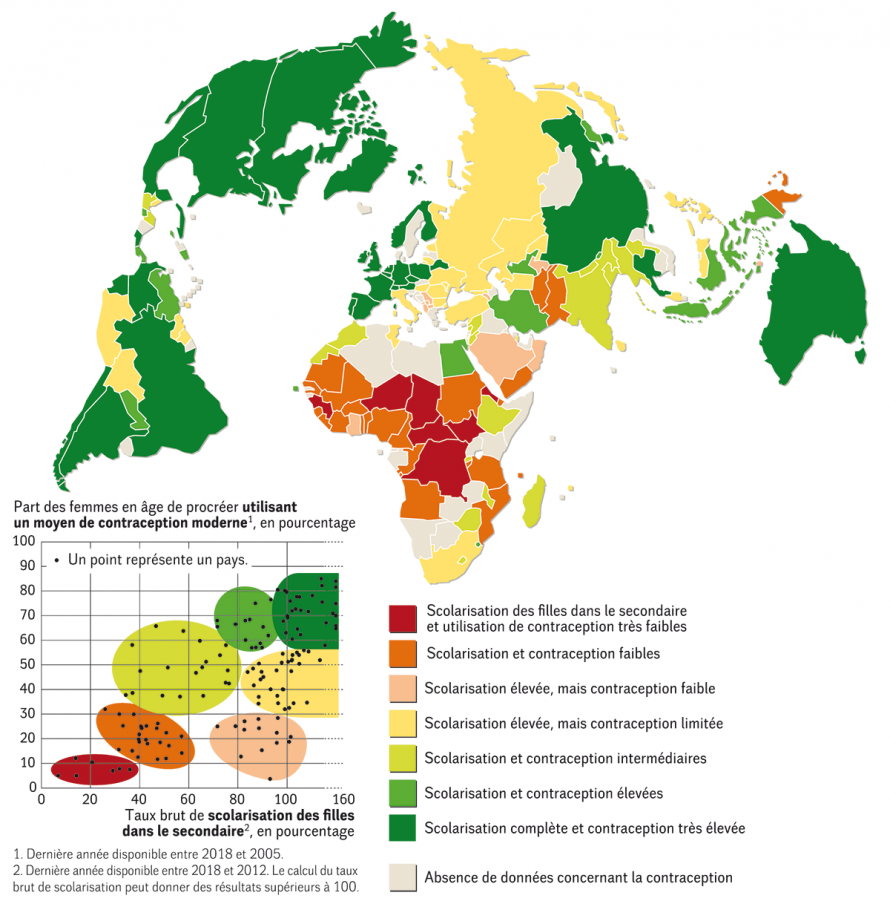
\includegraphics[width=0.475\textwidth]{fig1.png}	
\end{center}
\end{frame}
%------------------------------------------------
\begin{frame}[t]{El caso de la ley de aborto en Uruguay}
Dejando un poco el debate sobre la moralidad del aborto, es necesario saber qué tanto o cómo estas políticas crean un impacto.  
\begin{itemize}
	\item Por un lado, esto se relaciona con fecundidad (adolescente). 
	\item Esto podría conllevar impactos en educación y en el mercado laboral, sobre todo en familias de bajos ingresos. 
	\item ¿Qué otros impactos podrían haber? 
\end{itemize}
\end{frame}
%------------------------------------------------
\begin{frame}[t]{La Ley de aborto en Uruguay} 
En Latinoamérica: 
\begin{itemize}
	\item Altos niveles de fecundidad en general, sobre todo en adolescentes. 
	\item Poca educación en salud sexual y reproductiva. 
	\item En Nicaragua, 92 embarazos por mil adolescentes (UNFPA, 2018). La cuarta más alta en América. 
\end{itemize}
Uruguay: 
\begin{itemize}
	\item 2012: "Estrategia intersectorial y nacional de prevención del embarazo no intencional". 
\end{itemize}
\end{frame}
%------------------------------------------------
\begin{frame}[t]{Ley del aborto en Uruguay}
	Consecuencias de un embarazo adolescente (desde el punto de vista teórico): 
	\begin{itemize}
		\item Se pueden presenter peores resultados socioeconómicos (educativos), 
		\item dificultades en la permanencia en el sistema educativo, 
		\item mayor carga en el trabajo doméstico, y de cuidados, 
		\item presencia en el mercado laboral en temprana edad. 
	\end{itemize}
\end{frame}
%------------------------------------------------
\begin{frame}[t]{Ley del aborto en Uruguay}
	Esto a su vez, presenta desafíos metodológicos: 
	\begin{itemize}
		\item Problema de endogeneidad. 
		\item Causalidad inversa. 
		\item Sesgo de selección y variables omitidas. 
	\end{itemize}
	Las madres adolescentes difieren de sus pares en factores no-observables. ¿Qué factores? 
\end{frame}
%------------------------------------------------
\begin{frame}[t]{Alzúa y Velázquez (2018): Metodología}
\textbf{Objetivo}: Ver el impacto de fecundidad adolescente en los efectos educativos: 
\begin{itemize}
	\item Variable instrumental para contrarrestar endogeneidad. 
	\begin{itemize}
		\item IVE: grado de implementación de la ley, a partir de la tasa de aborto legal, en una región y determinado tiempo. 
		\item Esto instrumenbtalizada fecundidad en la región $ j $ en periodo $ t $. 
	\end{itemize}
	\item Datos a nivel región para asegurar confiabilidad. 
	\item Se omiten abortes ilegales. 
\end{itemize}
\end{frame}
%------------------------------------------------
\begin{frame}[t]{Resultados}
\vspace*{-2ex}
\begin{center}
	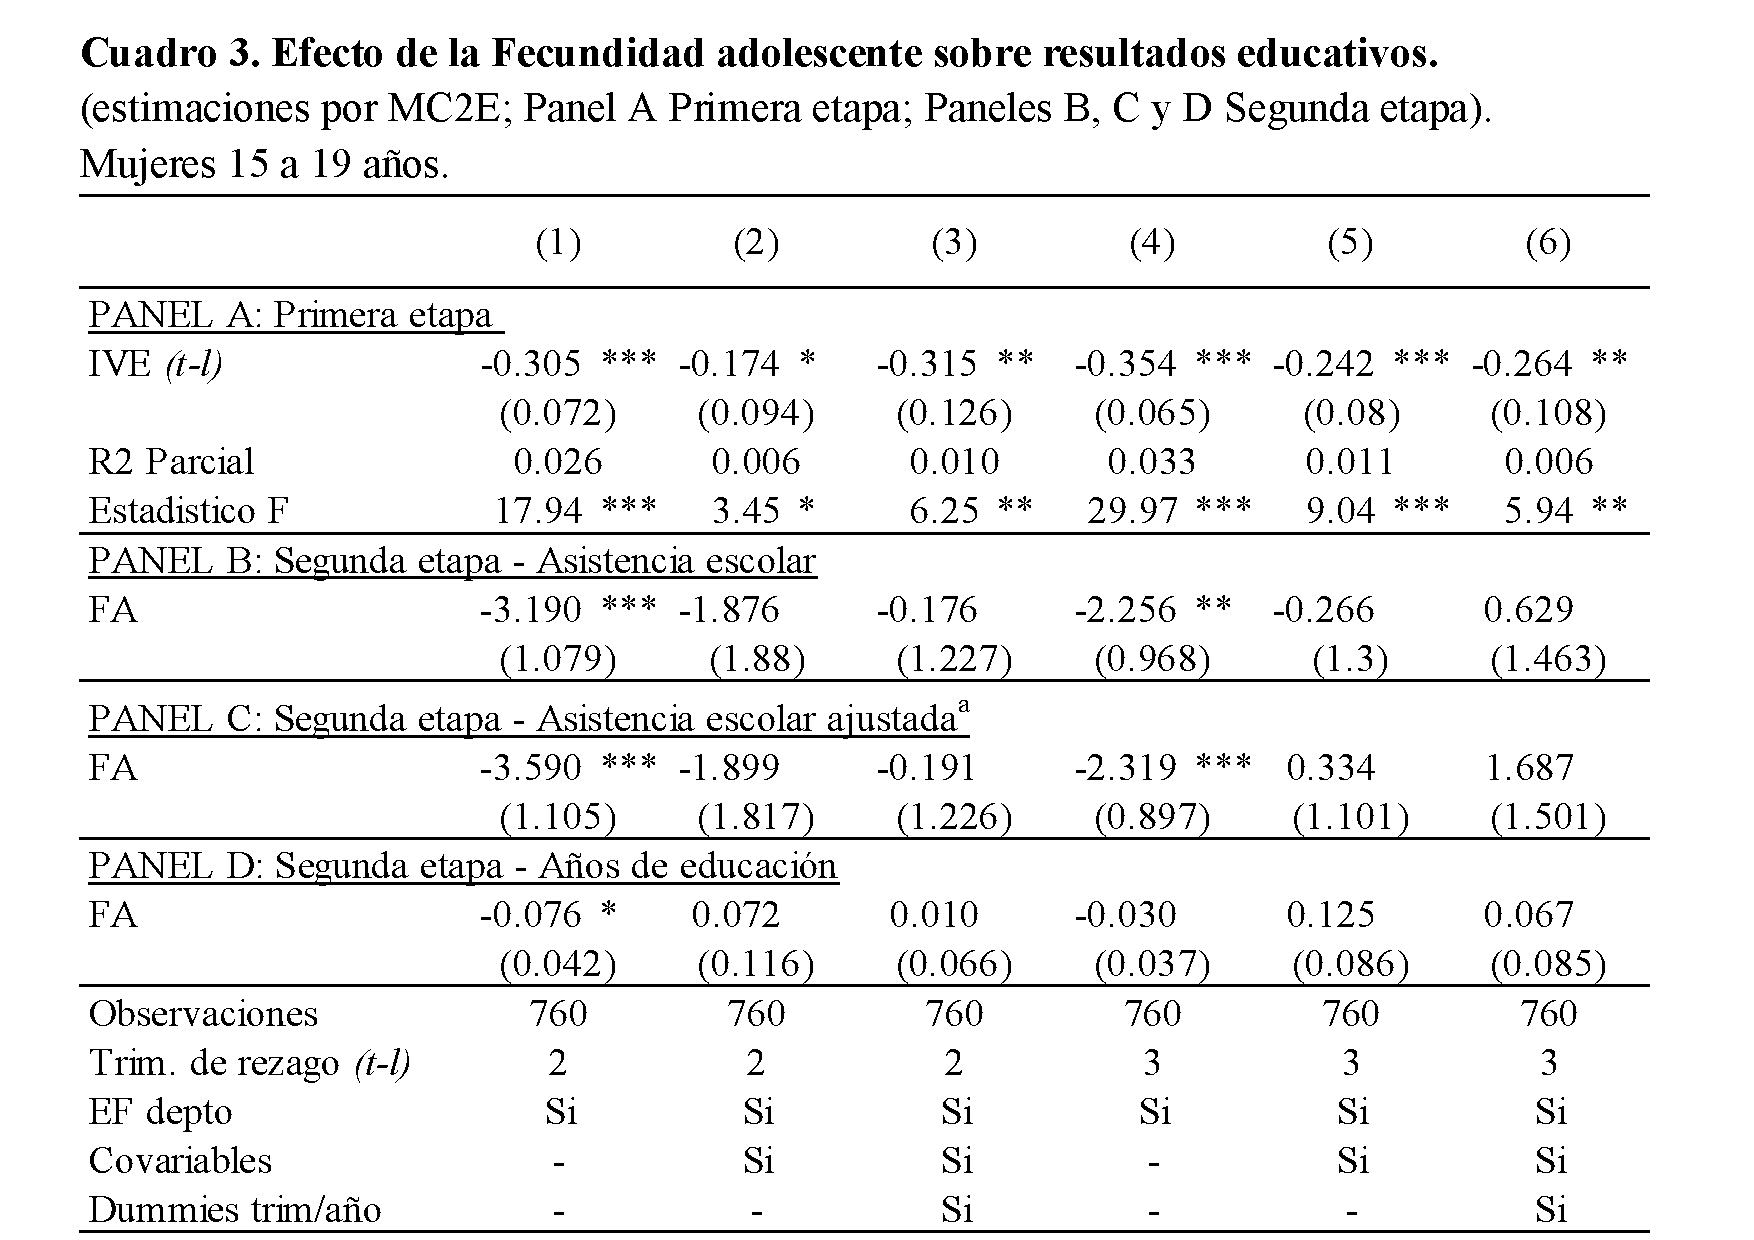
\includegraphics[width=0.7\textwidth]{tab3}
\end{center}
\end{frame}
%------------------------------------------------
\begin{frame}[t]{Reflexiones finales}
\begin{itemize}
	\item Los resultados sugieren que la legalización del aborto en Uruguay redujo la tasa de
	fecundidad adolescente. 
	\item Acceso al aborto con garantías legales y sanitarias contribuyó a debilitar las
	barreras para las jóvenes que cursan un embarazo no deseado. 
	\item No encuentran efecto en educación. 
	\item ¿Por qué creen que pasa esto? 
\end{itemize}
\end{frame}
%------------------------------------------------
%------------------------------------------------
\section{Anuncios}
\subsection{Anuncios}
%------------------------------------------------
\begin{frame}{Anuncios}
	
\end{frame}
%==============================================================
% END
%==============================================================
\miniframesoff 	
\begin{frame}[plain, standout]
Nos vemos la siguiente semana. 
\end{frame}
%------------------------------------------------
\end{document}		
